
\documentclass[submit,techrep,noauthor]{ipsj}


\usepackage[dvipdfmx]{graphicx}
\usepackage{latexsym}
\usepackage{url}
\usepackage{xcolor}
\usepackage{listings}
\usepackage{amsmath,amssymb}


% コード例を載せるためのあれこれ
\definecolor{lightred}{RGB}{255,230,230}
\definecolor{lightgreen}{RGB}{230,255,230}

\lstset{
basicstyle=\small\ttfamily,
abovecaptionskip=0pt,
captionpos=b,
frame=tb,
framexleftmargin=2em,
numbers=left,
numberstyle={\scriptsize},
xleftmargin=\parindent,
escapechar=| 
}

%ListingのキャプションがFigureになってしまうのをListingに直すコマンド
\usepackage{caption}
\makeatletter
\let\MYcaption\@makecaption
\makeatother
\usepackage{caption}
\makeatletter
\let\@makecaption\MYcaption
\makeatother

\newcommand{\todo}[1]{\colorbox{yellow}{{\bf TODO}:}{\color{red} {\textbf{[#1]}}}}
\newcommand{\ihara}[1]{\colorbox{green}{{\bf IHARA}:}{\color{blue} {\textbf{[#1]}}}}

\def\Underline{\setbox0\hbox\bgroup\let\\\endUnderline}
\def\endUnderline{\vphantom{y}\egroup\smash{\underline{\box0}}\\}
\def\|{\verb|}
%

\def\Underline{\setbox0\hbox\bgroup\let\\\endUnderline}
\def\endUnderline{\vphantom{y}\egroup\smash{\underline{\box0}}\\}
\def\|{\verb|}

\begin{document}


\title{CodeQLを用いた繰り返し処理を含む
\\
低速コードパターン検出手法
}

\noindent\ihara{このラベルは確認後に決して良い}

\noindent\todo{このラベルは解決後に消して良い}

\affiliate{WA}{和歌山大学\\
Wakayama University}

\author{野口 隼杜}{Noguchi Hayato}{WA}[s276185@wakayama-u.ac.jp]
\author{野口 朋弥}{Noguchi Tomoya}{WA}[s266227@wakayama-u.ac.jp]
\author{伊原 彰紀}{Ihara Akinori}{WA}[ihara@wakayama-u.ac.jp]

\begin{abstract}
% ソフトウェアの性能効率化は品質に直結する重要な課題であるが,ソースコード中に複数検出される性能ボトルネックの中から修正箇所を選定することは,開発者の経験に大きく依存している.また,プロファイラなどの動的解析ツールは,プログラムがある程度実装された後にしか適用できず,開発早期での性能改善作業を困難にしている.
% CodeQLによる静的解析を活用した繰り返し処理を含む低速コードパターンの早期検出手法を提案する.まず,プログラムの実行速度を比較するマイクロベンチマークを利用し,実行速度に差のある実装対から低速の原因となるコードパターンを作成する.次に,このコードパターンを基に,静的解析エンジンであるCodeQLのためのカスタムクエリを作成し,ソースコード中から該当する低速パターンを開発の早期段階で検出する.さらに,検出された箇所の依存関係を解析することで,修正が全体に与える影響や修正の優先度を推定する可能性についても言及し、より効果的な高速化修正候補の特定を目指す.ケーススタディを通じて,作成するコードパターンによる検出精度を評価するとともに,マイクロベンチマークを起点とする早期の性能改善アプローチの有用性について考察する.
\ihara{長すぎなので短くした.}
本研究では,マイクロベンチマークにおいて実行速度の比較で得られた低速ソースコード片をパターン化し,ソフトウェアに含まれる全てのソースコードの中から修正することでより高速なソースコードに修正できる可能性を有するソースコードを検出する手法を提案する.具体的には,静的解析エンジンCodeQLを用いることで,入出力は異なっていたとしても,特定の構造を有するソースコード片を検出することができる.ただし,\todo{課題が2つぐらいある?CodeQLへのクエリの作り方,出力結果にノイズが入る?}.本研究では,ケーススタディとして\todo{XXを対象として,評価実験を行った結果,XXがわかった.}
% 課題:「低速コードの特徴」をクエリにうまく反映させること・(そもそもCodeQLがセキュリティ用だから)カスタムクエリによる検出結果の評価および妥当性の検証方法が不明であること
\end{abstract}


\maketitle

%%%%%%%%%%%%%%%%%%%%%%%%%%%
%1
\section{はじめに}
%%%%%%%%%%%%%%%%%%%%%%%%%%%

 ソフトウェアの性能効率性は,ユーザ体験や運用コスト,さらにはシステム全体の品質に直結する重要な要素である\cite{performance1}\cite{performance2}\cite{negative}.性能効率性を向上するための方策として,ソフトウェア開発者は計算機能力やシステム設計の改善だけではなく,部分的なソースコードの最適化を積み重ねることで実現することもある.Webアプリケーション開発では,数行のソースコード修正によって最適化した結果,プログラムの実行時間が25\%から70\%高速化している\cite{jsRefac}.

性能効率性を向上するためのプログラム変更は,実装が進行するにつれて複雑になりやすい\cite{complicate}.また,保守性や可読性など,他のプログラム品質に否定的な影響を与えることもある\cite{negative}.したがって,性能効率性を向上するソースコードへ書き換えるためには,開発者に対して広範な知識や経験を要する.そのため,ソフトウェアの性能効率性を,実装途中の早期の段階で見積もり,性能低下の原因となるボトルネックを検出することは,性能効率性の改善にかかる修正工数を小さくできる\todo{できれば引用}. 

ソフトウェアの性能効率性を評価する方法として,プロファイラなどの動的解析ツールが広く用いられている.動的解析ツールは,実行時の関数呼び出しやリソース使用状況を精緻に観測し,性能低下の原因となる箇所の特定することができる.しかし,動的解析ツールによる性能効率性の評価は,評価対象の機能が実行できるまで実装が進んだ状態でなければ評価できないため,開発途中に性能効率性を評価することは難しい.

実装途中においても,部分的なソースコードの性能を定量的に評価する手法として,マイクロベンチマークを使用することができる.マイクロベンチマークは機能的に等価な複数の異なるソースコード片に対して実行時間を測定することで,ソースコード間の性能効率性を比較できる.ここで,マイクロベンチマークを共有するサービスとしてJavaScriptを対象とした,JsPerf\footnote{JsPerf: \url{https://jsperf.app/}}やMeasureThat.net\footnote{MeasureThat.net: \url{https://measurethat.net/}}がある.これらのサービスでは,ブラウザ上でマイクロベンチマークの実行環境を提供しており,JavaScriptのソースコード片の実行速度の測定および比較ができる.また,評価されたソースコード片,および測定結果はサービス上で公開されている.

開発者はマイクロベンチマーク共有サービスを用いて複数の実装方法を比較することはもちろん,サービス上でマイクロベンチマークを証拠としてソースコードの改善案を作成している事例もある\cite{saiki}.
しかし,開発者が,マイクロベンチマーク共有サービスで評価されたベンチマークに基づいて,性能効率性が向上できる箇所の検出および,その修正を行うためには,実装するソフトウェアにおける,ソースコード間の依存関係や構造に影響するため開発者の知識や技量に依る.特に,ソフトウェア中に性能効率性が向上できる箇所が複数存在する場合,優先的に修正する箇所の特定は容易でない.

%しかし,マイクロベンチマークをどう設計するか,マイクロベンチマークの結果をどう解釈するかは,性能効率性向上のためのプログラム変更と同様に,開発者の技量に依るところが大きい.さらに,どの箇所を対象にマイクロベンチマークの結果を適用すべきかを判断するには,事前に潜在的な低速箇所を特定する必要がある.
% 複数の性能問題が存在する場合には,これらに加えて,どの箇所を優先的に修正すべきかの判断も必要となるが,プログラム全体の依存関係や構造が大きく影響するため,効率的な性能改善作業を体系的に行うことは容易ではなく,マイクロベンチマークの利用における課題となっている.

% ソースコード「片」で統一
本研究では,ソフトウェア中に潜在する,修正することで性能効率性,特に実行速度の向上が期待されるソースコード片の検出を目的とする.具体的には,マイクロベンチマーク共有サービスで提供されるマイクロベンチマークで比較されたソースコード片の構造差分から低速コードパターン\todo{高速コードパターンも抽出できるけど...言い方考える}を作成する.これを利用し,静的解析エンジンCodeQL\footnote{\url{https://codeql.github.com/}}\cite{ql}を用いて,ソースコード中から低速なソースコード箇所を検出する.CodeQLは,マイクロベンチマーク共有サービスで公開されるソースコード片とは入出力が異なっていても,構造が類似するソースコードを検出が期待される.
\todo{また,検出された箇所に対して依存関係を解析することで,修正がプログラム全体に与える影響や修正の優先度を推定する可能性についても検討する.}\ihara{$\leftarrow$ここは結果次第で記述するか要検討}提案手法は,動的解析に依存せずに潜在的な性能効率性に寄与するボトルネックを実装初期段階で検出できる.
% ,修正効果の高い箇所を効率的に見出すことを目指す.

続く\ref{sec:background}章では,本研究で利用するマイクロベンチマーク共有サービスにおけるマイクロベンチマークの特徴,および関連研究を紹介し,本研究の立ち位置を述べる. \ref{sec:pre-analysis}章で事前分析について示し, \ref{sec:approach}章では,本研究の提案手法を述べ,\ref{sec:case-study}章において,ケーススタディの結果を述べる.\ref{sec:discussion}章で考察を行い,\ref{sec:summary}章で本研究をまとめる. 


%%%%%%%%%%%%%%%%%%%%%%%%%%%
%2
\section{マイクロベンチマークに基づく性能ボトルネック検出\todo{大きく修正が必要なため,ここは後で確認する}}
\label{sec:background}
%%%%%%%%%%%%%%%%%%%%%%%%%%%

%2.1
\subsection{マイクロベンチマーク共有サービス}

%----------------------
\begin{figure}[t]
    \centering
    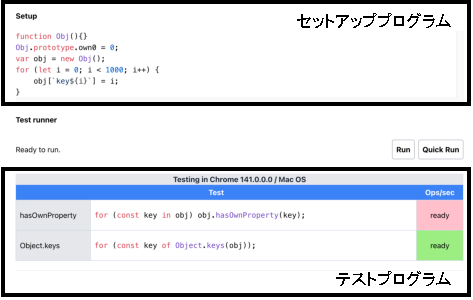
\includegraphics[width=1.0\linewidth]{./Noguchi_fig/jsPerf_example.pdf}
    \caption{マイクロベンチマーク共有サービスの投稿例\protect\footnotemark}
    \label{fig:jsPerf}
\end{figure}

\footnotetext{\url{https://jsperf.app/qiwudo}}
%----------------------

マイクロベンチマーク共有サービスは,開発者がプログラムの実行速度を比較・共有するためのオンラインサービスである.図\ref{fig:jsPerf}に,マイクロベンチマーク共有サービスの1つであるjsPerf上で実際に投稿されているマイクロベンチマークの例を示す.

マイクロベンチマーク共有サービスにおける各投稿は,1つのセットアッププログラムと,1つ以上のテストプログラムから構成される.図上部に示すセットアッププログラムでは,検証対象のコードで共通して利用される変数の初期化やデータの準備が行われる.一方,図下部に示すテストプログラムでは,同一の機能を異なる方法で実装したプログラム(大抵は短いソースコード片)が複数提示され,それぞれの実行速度を計測・比較できる.
このようなマイクロベンチマークは,データ構造や制御構文の選択,メソッド呼び出しの方法などに多様性が見られることが特徴であり,実行速度の差とその要因となる実装方法を捉えることができる.本研究では,このようなマイクロベンチマーク共有サービス上の実装対を分析し,性能効率性,特に実行速度に影響を与える構造的特徴を分析および抽出するために利用する.


% マイクロベンチマーク共有サービスの一つであるjsPerfにおいて,実際に投稿されているマイクロベンチマークの例を図\todo{スクショ挿入・リンクをフットノート}に示す,マイクロベンチマーク共有サービスでは,1つの検証における準備を行うセットアッププログラムと,検証対象となる2つ以上のテストプログラムから構成されている.図上部に示すプログラムがセットアッププログラムを示しており,検証対象のプログラムで利用される変数の初期化などが行われている.図下部に示すプログラムがテストプログラムを示しており,図では,\todo{コードの説明}と\todo{同じく}の実行速度が計測・比較検証される.

% マイクロベンチマーク共有サービスでは,図に示すような実装対が保存・公開されており,同一の機能を異なる方法で実装した非常に短いコードの対によって構成されており,データ構造や制御構文,使用するメソッドの選択などに多様性が見られる.


%2.2
\subsection{関連研究}

Selakovic ら\cite{jsRefac}は,JavaScript プロジェクトにおいて,開発者が高速化のために行ったリファクタリングを調査した.その結果,開発者は10行程度の小さい範囲の修正によって高速化への対処を行なっていることを明らかにした.この結果は,マイクロベンチマーク共有サービスに見られる,短いコードによる高速化への利用可能性を示すものとして,本研究の動機づけとなっている.また,\cite{jsRefac}は,JavaScript プロジェクトの解析によって 10 件の頻出する高速化改良パターンを作成している.この改良パターンを用いた自動修正は一定の高速化効果を示しているが,該当箇所の特定における制約などから,広範な適用には至っていない.

Turcotte ら\cite{DrAsync}は,JavaScript 言語における非同期処理に注目した性能アンチパターンを定義し,静的解析エンジンであるCodeQL\cite{ql}を利用したアンチパターンの検出と,動的解析を利用したパフォーマンスの監視を組み合わせ,修正可能な性能アンチパターンの検出を行った.本研究の静的解析による低速コードパターンの検出はこれに着想を得ている.

大森ら\cite{omori}は,マイクロベンチマーク共有サービスで公開される実行速度が向上するプログラムを収集し,これをデータセットとして大規模な言語学習モデルをファインチューニングすることで,実行を高速化するプログラムに自動リファクタリングするモデルを作成した.この結果,マイクロベンチマーク共有サービス上のプログラムに対しては,ChatGPT-4o より約3倍のリファクタリングに成功している.しかし,適用対象がマイクロベンチマーク共有サービス上のプログラムに留まっており,\cite{jsRefac}と同様,広範な適用には至っていない.

本研究では,繰り返し処理に注目し,マイクロベンチマーク共有サービスで公開される実装対における低速コードから,構造的差分に基づいて低速コードパターンを抽出し,静的解析を用いた性能ボトルネックの早期検出を行うとともに,適用範囲を拡張する上での検出精度の指標について議論する.\todo{あいまい...もっといい表現があるはず}


%%%%%%%%%%%%%%%%%%%%%%%%%%%
%3
\section{事前分析}
\label{sec:pre-analysis}
%%%%%%%%%%%%%%%%%%%%%%%%%%%


本研究では,大森ら\cite{omori}が作成した,マイクロベンチマーク共有サービスjsPerfにおける,実行速度に有意差があり,外的振る舞いが等しいことが検証された実装対29,809件を利用する.以降,この実装対をマイクロベンチマーク実装対とし,各実装対において,実行速度が遅いコードを低速コード,実行時間が速いコードを高速コードとする.

%3.1
\subsection{繰り返し処理を含むマイクロベンチマーク実装対}
\label{section3.1}

% \todo{図1で示すように} 繰り返し処理を含む実装対が全体の約43%(12,948対)存在する.

マイクロベンチマーク実装対を目視調査した結果,実装対の両方もしくは片方に繰り返し処理を含むものが多く存在することが確認された.特に,巨大な配列や長大な繰り返し処理を用いて性能差を強調する実装対や,繰り返し処理自体の違いによって実行時間に差が生まれる実装対など,複数の傾向が確認された.

このような観察結果から,本研究ではマイクロベンチマーク実装対に対して繰り返し処理構造に着目した特徴分析を行うこととした.対象とする繰り返し処理は,JavaScriptにおける for,for-of,for-in,while,および do-while 構文である.

分析にあたっては,各実装対のソースコードを GumTree \cite{gumtree}により抽象構文木へと変換し,実装対の抽象構文木間の差分解析を行った.差分解析の結果に対して,(1) 差分が直接繰り返し処理構造を含むか,および (2) 差分要素の構造的な親要素に繰り返し処理が含まれるかを確認事項とし,繰り返し処理に関連する差分要素として収集した.抽出された箇所に応じて目視で確認を行い,実装対の構造的特徴および性能差との関係を整理した.
この分析の結果,マイクロベンチマーク実装対には繰り返し処理について,いくつかのパターンが存在することが明らかとなった.Listing~\ref{diff-inloop},Listing~\ref{diff-loop},Listing~\ref{diff-method}に,特徴となる部分について示す.

Listing~\ref{diff-inloop}は,それぞれfor文内で concat メソッド, push メソッドを用いている実装対である.これは,繰り返しの構造は一致しているが,繰り返し内部で実行する処理が異なるパターンである.
%----------------------------------
\begin{lstlisting}[caption=Pairs with differences within the loop, label=diff-inloop, captionpos=t]
// slow
for (var VAR_2 = 0; VAR_2 < 5000; VAR_2++)
    VAR_1 = VAR_1.concat([\"1\", \"2\"]);

// fast
for (var VAR_2 = 0; VAR_2 < 5000; VAR_2++)
    VAR_1.push(\"1\", \"2\");
\end{lstlisting}
%----------------------------------

Listing~\ref{diff-loop}は,それぞれ,for-in文を用いて配列の全要素にアクセスする実装と,同様の処理をwhile文で実装したものである.ここで示すパターンは実行時間の差が,繰り返し処理自体の違いに起因するパターンである.
%----------------------------------
\begin{lstlisting}[caption=Pairs with loop differences, label=diff-loop, captionpos=t]
// slow
for (var VAR_2 in VAR_1) {
    VAR_1[VAR_2];
}

// fast
var VAR_3 = 0;
while (VAR_3 < VAR_1.length) {
    VAR_1[VAR_3];
    VAR_3++;
}
\end{lstlisting}
%----------------------------------

Listing~\ref{diff-method}は,繰り返し処理をforEachメソッドで実装したものとfor-of文で実装したものである.これは,メソッドによる処理とそれに代替する繰り返し処理について比較したパターンである.
%----------------------------------
\begin{lstlisting}[caption=Pairs of Method and alternative loop, label=diff-method, captionpos=t]
// slow
var VAR_5 = new Set(VAR_2);
VAR_5.forEach(VAR_6 => {});

// fast
for (let VAR_7 of VAR_2) {}
\end{lstlisting}
%----------------------------------

これらの結果から,マイクロベンチマーク実装対には繰り返し処理の構造および繰り返し内部の操作内容の違いが性能差の要因の1つとして存在することが確認された.本研究では,このような繰り返し処理に関する差分構造を低速コードの特徴として抽出し,次章で述べる低速コードパターンの抽出および静的検出に利用する.


%%%%%%%%%%%%%%%%%%%%%%%%%%%
%4
\section{CodeQLクエリを用いた低速コードパターン検出手法}
\label{sec:approach}
%%%%%%%%%%%%%%%%%%%%%%%%%%%

%----------------------
\begin{figure*}[t]
    \centering
    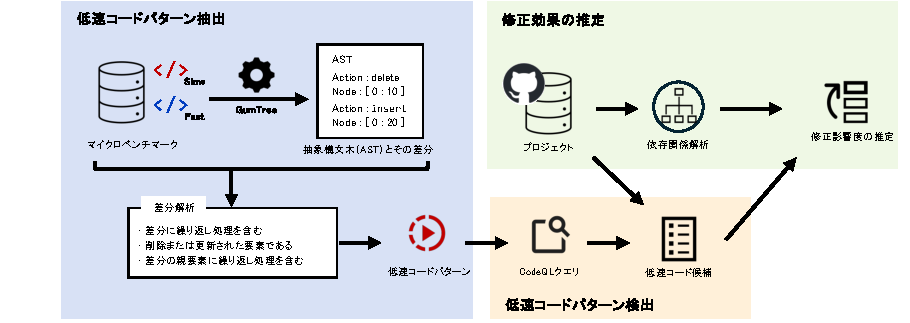
\includegraphics[width=1.0\linewidth]{./Noguchi_fig/approach_abst.pdf}
    \caption{本研究の全体像\todo{差し替える}}
    \label{fig:Approach}
\end{figure*}
%----------------------

本研究では,実行速度の向上が期待されるソースコード片の検出に向けて,
マイクロベンチマーク共有サービスで提供される,実行速度の比較されたソースコード片の構造差分から低速コードパターンを作成する.これを利用し,静的解析エンジンCodeQLを用いて,ソースコード中から低速なソースコード片を検出する.図\ref{fig:Approach}は,本研究で提案する手法の概略図を示す.本手法は3つの方法で構成し,それぞれについて述べる.
% (1) マイクロベンチマーク実装対より,低速コードの特徴を実装対の構造的差分から抽出し,低速コードパターンを作成する.作成したパターンをもとに静的解析エンジンCodeQL\cite{ql}を用いて,ソースコード中の低速コードを静的に検出する手法を提案する.また,検出結果について,修正効果の高い箇所をプログラム中の依存関係の数から推定する.以降でその詳細を述べる.


%4.1
\subsection{分析対象ベンチマークの収集}

\ref{sec:pre-analysis}節で述べたように,著者らはマイクロベンチマーク共有サービスにおいて,繰り返し処理の構造および繰り返し内部の操作内容の違いが性能差の要因の1つであることを確認した.本研究では,従来研究で対象とするベンチマークの中で,ベンチマークで比較されるソースコード間で,繰り返し処理の構造,および繰り返し内部の操作内容に違いを含むベンチマークを分析対象とする.\todo{プログラムとして正規表現があるのでは?forとかwhileとか。。。?ベンチマークのタイトルとか?}


%4.2
\subsection{低速コードのパターン作成}
本研究はベンチマークに含まれる低速コードから高速コードへの変更を仮定して,その構造的差分からパターンを作成する.差分抽出には,ソースコードの抽象構文木に基づいた比較が可能である差分解析器 GumTree\cite{gumtree} を使用する.GumTree によって得られた構造的差分のうち,低速コードから削除または更新された要素を抽出する.これらの要素は,高速コードに存在しない要素であり,低速コード特有の処理や構造を示す要素であると考えられるため,低速コードの特徴候補として収集する.収集した低速コードの特徴候補の中には,繰り返し処理の条件,メソッド呼び出し,および配列・オブジェクト操作などの意味的に有効な要素\todo{選別というなら「など」という曖昧な表現は使わず,すべて書く}を含む.

% 具体的には,ベンチマークに含まれる低速コードから高速コードへの変更を仮定し,繰り返し処理の構造および繰り返し内部の操作内容が削除または更新されるベンチマークを対象とする.ここで,削除・更新される要素は,低速コードにのみ含まれる要素であることから,低速コードの特徴がその中に含まれることを期待している\todo{例えばListing1では〜 具体例のせて後で表現直す}.ソースコード差分解析器には,ソースコードの抽象構文木に基づき比較しているGumTree\cite{gumtree}を使用する.

% GumTreeが,繰り返し処理の条件の削除,または更新として検出したノードを取得する.これらのノードは,低速コードにのみ含まれる実装方法であり,対応する高速コードに対して,低速コード特有の処理構造を示すものであるため,低速コードパターンの候補とする.\todo{直前2行がいるか悩む.}
% 次に,取得したノードにおいて,使用されているメソッド呼び出しや配列・オブジェクト操作の形態および,それらの位置情報をもとに,低速コードパターンを特定する.

抽出した低速コードの特徴要素は,それぞれのベンチマークで比較されたソースコードにおける行番号や階層情報から\todo{何を?}統合することで,低速コードパターンを形成する.例えば,for文ノードと,その配下にあるメソッド呼び出しノードを関連づけることで「forループ内でのメソッド呼び出し」のような具体的なパターンを作成する.こうして得られた構造は,複数の実装対に共通して出現する低速コード特有の構文的特徴を表す.\todo{具体例がないとわからない.}

%4.3
\subsection{低速コードパターンの検出}

本研究では,作成した低速コードパターンに基づく検索クエリを作成し,静的解析ツールCodeQL\cite{ql}を用いて低速なソースコード片を検出する.CodeQLは,GitHubが主にセキュリティ検査を自動化する目的で開発されたコード分析ツールである.具体的には,分析対象とするプログラムから抽象構文木,データフロー情報,型情報,呼び出し関係などをデータベースに保持する.このデータベースに対して,SQLライクなクエリ言語を用いて,特定の構造や振る舞いを持つソースコード検索を実現している.
% ソースコード中に含まれる低速コードを静的に検出する手法について述べる.本研究では,\cite{DrAsync}に着想を得て,低速コードパターンを検出するための静的解析ツールとして CodeQL\cite{ql} を用いる.
% CodeQLは,GitHub が開発した,主にセキュリティ検査を自動化する目的で開発されたコード分析ツールであり,プログラムから抽象構文木の構築とデータフローの抽出を行い,それらをデータベースとして保持する.このデータベースに対して,SQL ライクなクエリ言語を用いて検索を行うことで,特定の構造や振る舞いを持つコード断片を効率的に抽出できる.
本研究では,低速コードパターンをもとにCodeQLに対応するクエリを作成し,ソースコード内で同様の構造を持つ箇所を検出する.\todo{低速コードパターンの実例使って,クエリも載せること}

% クエリの作成には,マイクロベンチマーク実装対に適用し,その検出精度を検証するとともに,元となった低速パターンを含む低速コードを検出できるよう調整を行った.また,それ以外で検出された低速コードについても,目視で確認し,クエリの妥当性を検証した.最終的に作成したクエリを,元となった実装対とともに\todo{図}に示し,ケーススタディにおける低速コードパターンの検出に利用する.


%4.4
\section{評価方法\todo{ここは結果を見てから直す}}

本研究では,提案手法の有効性を検証するために,低速コードパターンの検出結果に対し,\todo{評価方法は仮}構造的類似度と意味的類似度の両側面から評価を行う.

\todo{使う指標の説明}
構造的類似度は\todo{指標1}を用いて算出し,元コードとの構造的差異を捉える.一方,意味的類似度は\todo{指標2}を用いて算出し,元コードとの処理内容の差異を捉える.

具体的には,検出結果の中から無作為に\todo{n}件を選択し,低速コードパターンの元となった実装対との類似度を算出する.次に,目視により各検出箇所が,クエリの元となったマイクロベンチマーク実装対における低速コードの特徴を正しく捉えているかを確認する.
各類似度指標と目視確認結果と照らし合わせることで,どの指標・閾値設定が低速コード検出に最も有効であるかを議論する.


\ihara{ここまで修正済み}

%%%%%%%%%%%%%%%%%%%%%%%%%%%
%5
\section{ケーススタディ}
\label{sec:case-study}
%%%%%%%%%%%%%%%%%%%%%%%%%%%

%5.1
\subsection{データセット}

ケーススタディとして,,プログラムバージョン管理システムであるGitHubで公開されている,主要言語がJavaScript,\todo{要検討}スター数が100以上,最終コミットが1年以内,\todo{要検討}クエリによる検出結果がn件以上のxプロジェクトを選定した.\todo{表}の左から1列目にプロジェクト一覧を示し,各プロジェクトの特徴量?統計量?を示す.

%5.2
\subsection{低速コードパターンの検出}


クエリの作成には,マイクロベンチマーク実装対に適用し,その検出精度を検証するとともに,元となった低速パターンを含む低速コードを検出できるよう調整を行った.また,それ以外で検出された低速コードについても,目視で確認し,クエリの妥当性を検証した.最終的に作成したクエリを,元となった実装対とともに\todo{図}に示し,ケーススタディにおける低速コードパターンの検出に利用する.

%5.3
\subsection{検出結果の類似度}




%%%%%%%%%%%%%%%%%%%%%%%%%%%
%6
\section{考察}
\label{sec:discussion}
%%%%%%%%%%%%%%%%%%%%%%%%%%%



%6.1
\subsection{検出結果}

低速コードパターンの抽出とクエリへのマッピングの流れ
広く検出できた話

%6.2
\subsection{類似度指標}

なぜその結果か
依存関係を見ることは意味があるか・他の指標は何か

\subsection{妥当性の脅威}

%6.1
\noindent\textbf{内的妥当性: }
クエリを手作業で作成した&その正確性は目視による調査であるため,低速コードパターンを本当に反映できているかは不明.小さくするためにマイクロベンチマークに実際に投げて確認はしている.
利用しているjsPerfはサービスを終了しているため,現在も高速な実装方法とは限らない.(大森研究でも同じ言及あり)
低速コードパターンは,GumTreeによる差分から作成しているため,差分でうまくとれていないせいで低速実装を表現したパターンとなっていない可能性.本研究においては,目視を通してパターンの元となった実装を確認してサンプルを作成しているからその心配は少ないけど,今後パターンを広げていく際には考慮しないといけない.今後の課題とする.

\noindent\textbf{外的妥当性: }
リポジトリの選定について,時間的制約上,スター数上位のものに絞った.そのため,結果の一般性は下がる.特に,スター数上位のものは,十分に保守されたソフトウェアであることが多く,本手法における検出および効果の大きい箇所の推定における影響は異なることが考えられる.

%%%%%%%%%%%%%%%%%%%%%%%%%%%
%7
\section{おわりに}
\label{sec:summary}
%%%%%%%%%%%%%%%%%%%%%%%%%%%

\begin{acknowledgment}
\todo{本研究は,JSPS における科研費(XXXX)}
\end{acknowledgment}



\bibliographystyle{ipsjunsrt}
\bibliography{bibnoguchi}

\end{document}
